% ===========================================================================
%  TikuOS — TikuKits DS: Sorted Array for Embedded Systems
%  Beamer Presentation
% ===========================================================================
\documentclass[aspectratio=169, 10pt]{beamer}

% ---- Theme ----------------------------------------------------------------
\usetheme{Madrid}
\usecolortheme{whale}
\setbeamertemplate{navigation symbols}{}
\setbeamertemplate{footline}{%
  \leavevmode\hbox{%
    \begin{beamercolorbox}[wd=.33\paperwidth,ht=2.5ex,dp=1ex,center]{author in head/foot}%
      \usebeamerfont{author in head/foot}\insertshortauthor
    \end{beamercolorbox}%
    \begin{beamercolorbox}[wd=.34\paperwidth,ht=2.5ex,dp=1ex,center]{title in head/foot}%
      \usebeamerfont{title in head/foot}\insertshorttitle
    \end{beamercolorbox}%
    \begin{beamercolorbox}[wd=.33\paperwidth,ht=2.5ex,dp=1ex,right]{date in head/foot}%
      \usebeamerfont{date in head/foot}\insertshortdate{}\hspace*{2em}%
      \insertframenumber{}/\inserttotalframenumber\hspace*{2ex}
    \end{beamercolorbox}}%
  \vskip0pt%
}

% ---- Packages -------------------------------------------------------------
\usepackage{listings}
\usepackage{graphicx}
\usepackage{hyperref}
\usepackage{booktabs}
\usepackage{multirow}
\usepackage{tikz}
\usetikzlibrary{arrows.meta, positioning, shapes.geometric, calc,
                decorations.pathreplacing, fit}
\usepackage{amsmath}

% ---- Code listing style ---------------------------------------------------
\lstset{
  basicstyle=\ttfamily\scriptsize,
  keywordstyle=\color{blue}\bfseries,
  commentstyle=\color{gray},
  stringstyle=\color{red!70!black},
  showstringspaces=false,
  breaklines=true,
  frame=single,
  rulecolor=\color{black!30},
  backgroundcolor=\color{blue!3},
  tabsize=4,
}
\lstdefinestyle{cstyle}{
  language=C,
  morekeywords={uint8_t,uint16_t,uint32_t,int32_t,int16_t,bool,
                tiku_kits_ds_sortarray_t,tiku_kits_ds_elem_t,
                TIKU_KITS_DS_OK,TIKU_KITS_DS_ERR_NULL,
                TIKU_KITS_DS_ERR_SIZE,TIKU_KITS_DS_ERR_FULL,
                TIKU_KITS_DS_ERR_EMPTY,TIKU_KITS_DS_ERR_NOT_FOUND,
                TIKU_KITS_DS_SORTARRAY_MAX_SIZE,
                NULL},
}

% ---- Metadata -------------------------------------------------------------
\title[TikuKits DS]{TikuKits DS: Sorted Array for Embedded Systems}
\subtitle{Simple. Ubiquitous. Intelligence, Everywhere.}
\author[Ambuj Varshney]{Ambuj Varshney \\ \texttt{ambuj@tiku-os.org}}
\date{\today}

% ===========================================================================
\begin{document}

% ---------------------------------------------------------------------------
\begin{frame}
\titlepage
\end{frame}

% ---------------------------------------------------------------------------
\begin{frame}{Outline}
\tableofcontents
\end{frame}

% ===========================================================================
\section{Motivation}
% ===========================================================================

\begin{frame}{Why a Sorted Array on MCUs?}
\begin{columns}[T]
\begin{column}{0.48\textwidth}
\begin{block}{Embedded Use Cases}
\begin{itemize}
  \item \textbf{Calibration thresholds} --- sorted ADC breakpoints
  \item \textbf{Alarm tables} --- ordered severity levels
  \item \textbf{Priority ranking} --- task or sensor priorities
  \item \textbf{Fast lookup} --- O($\log n$) binary search
\end{itemize}
\end{block}

\begin{block}{Constraints}
\begin{itemize}
  \item No heap allocation (static array)
  \item Tiny capacity (16 elements max by default)
  \item Insert/remove via \texttt{memmove} --- O($n$)
  \item Cache-friendly contiguous memory
\end{itemize}
\end{block}
\end{column}

\begin{column}{0.48\textwidth}
\begin{center}
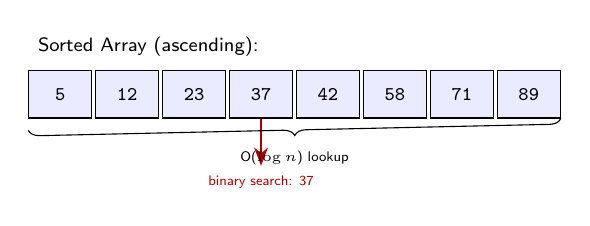
\begin{tikzpicture}[
    cell/.style={draw, minimum width=0.8cm, minimum height=0.6cm,
                 font=\scriptsize\ttfamily},
    >=Stealth
  ]
  \foreach \v [count=\i from 0] in {5,12,23,37,42,58,71,89} {
    \node[cell, fill=blue!8] (c\i) at (\i*0.85, 0) {\v};
  }
  \node[font=\scriptsize\sffamily, above=0.3cm of c0.north west, anchor=west]
    {Sorted Array (ascending):};

  % Binary search arrow
  \draw[->, thick, red!70!black] (c3.south) -- ++(0,-0.6)
    node[below, font=\tiny\sffamily] {binary search: 37};

  % Brace
  \draw[decorate, decoration={brace, mirror, amplitude=4pt}]
    (c0.south west) ++(0,-0.15) -- (c7.south east) ++(0,-0.15)
    node[midway, below=6pt, font=\tiny\sffamily] {O($\log n$) lookup};
\end{tikzpicture}
\end{center}

\vspace{0.5em}
\begin{alertblock}{Design Goal}
A statically allocated array that \textbf{automatically maintains
ascending order}. Binary search for O($\log n$) lookups, element
shifting for inserts and removes. No pointers, no heap.
\end{alertblock}
\end{column}
\end{columns}
\end{frame}

% ===========================================================================
\section{Algorithm Theory}
% ===========================================================================

\begin{frame}{Sorted Array Operations}
\begin{columns}[T]
\begin{column}{0.48\textwidth}
\textbf{Insert (value = 35):}
\begin{enumerate}
  \item Binary search for insertion position
  \item \texttt{memmove} elements right by one
  \item Place new element at found position
\end{enumerate}

\vspace{0.5em}
\begin{center}
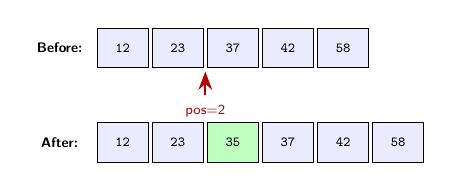
\begin{tikzpicture}[
    cell/.style={draw, minimum width=0.65cm, minimum height=0.5cm,
                 font=\tiny\ttfamily},
    >=Stealth
  ]
  % Before
  \node[font=\tiny\sffamily\bfseries] at (-0.8, 0.5) {Before:};
  \foreach \v [count=\i from 0] in {12,23,37,42,58} {
    \node[cell, fill=blue!8] (b\i) at (\i*0.7, 0.5) {\v};
  }

  % Arrow showing insertion point
  \draw[->, thick, red!70!black] (1.05, -0.1) -- (1.05, 0.2)
    node[below=0.3cm, font=\tiny\sffamily] {pos=2};

  % After
  \node[font=\tiny\sffamily\bfseries] at (-0.8, -0.7) {After:};
  \foreach \v [count=\i from 0] in {12,23,35,37,42,58} {
    \pgfmathsetmacro{\fillcol}{\i == 2 ? "green!25" : "blue!8"}
    \node[cell, fill=\fillcol] (a\i) at (\i*0.7, -0.7) {\v};
  }
\end{tikzpicture}
\end{center}

\vspace{0.5em}
\textbf{Complexity:}
\begin{itemize}
  \item Search: O($\log n$)
  \item Insert: O($\log n$) search + O($n$) shift
  \item Remove: O($\log n$) search + O($n$) shift
\end{itemize}
\end{column}

\begin{column}{0.48\textwidth}
\textbf{Remove (value = 37):}
\begin{enumerate}
  \item Binary search to find element
  \item \texttt{memmove} elements left by one
  \item Decrement size
\end{enumerate}

\vspace{0.5em}
\begin{center}
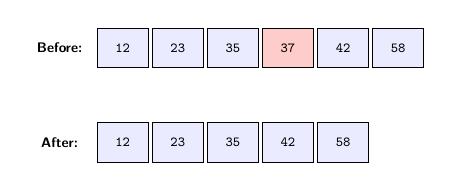
\begin{tikzpicture}[
    cell/.style={draw, minimum width=0.65cm, minimum height=0.5cm,
                 font=\tiny\ttfamily},
    >=Stealth
  ]
  % Before
  \node[font=\tiny\sffamily\bfseries] at (-0.8, 0.5) {Before:};
  \foreach \v [count=\i from 0] in {12,23,35,37,42,58} {
    \pgfmathsetmacro{\fillcol}{\i == 3 ? "red!20" : "blue!8"}
    \node[cell, fill=\fillcol] (b\i) at (\i*0.7, 0.5) {\v};
  }

  % After
  \node[font=\tiny\sffamily\bfseries] at (-0.8, -0.7) {After:};
  \foreach \v [count=\i from 0] in {12,23,35,42,58} {
    \node[cell, fill=blue!8] (a\i) at (\i*0.7, -0.7) {\v};
  }
\end{tikzpicture}
\end{center}

\vspace{0.5em}
\begin{block}{Duplicate Handling}
Duplicates are \textbf{allowed}. On insert, the new element is placed
\textbf{after} existing equal values (stable insertion). Binary search
finds the \emph{first} occurrence.
\end{block}
\end{column}
\end{columns}
\end{frame}

% ---------------------------------------------------------------------------
\begin{frame}{Binary Search Internals}
\begin{columns}[T]
\begin{column}{0.48\textwidth}
\textbf{Standard binary search (find):}
\begin{enumerate}
  \item Set \texttt{lo = 0}, \texttt{hi = size - 1}
  \item While \texttt{lo <= hi}:
  \begin{itemize}
    \item \texttt{mid = (lo + hi) / 2}
    \item If \texttt{data[mid] == key}: return \texttt{mid}
    \item If \texttt{data[mid] < key}: \texttt{lo = mid + 1}
    \item Else: \texttt{hi = mid - 1}
  \end{itemize}
  \item Not found: return \texttt{ERR\_NOT\_FOUND}
\end{enumerate}

\vspace{0.5em}
\textbf{Lower-bound search (insert position):}
\begin{enumerate}
  \item Set \texttt{lo = 0}, \texttt{hi = size}
  \item While \texttt{lo < hi}:
  \begin{itemize}
    \item \texttt{mid = (lo + hi) / 2}
    \item If \texttt{data[mid] <= key}: \texttt{lo = mid + 1}
    \item Else: \texttt{hi = mid}
  \end{itemize}
  \item Return \texttt{lo} --- the insertion point
\end{enumerate}
\end{column}

\begin{column}{0.48\textwidth}
\begin{center}
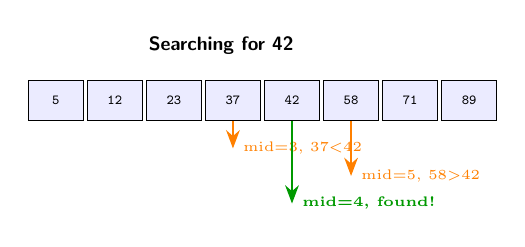
\begin{tikzpicture}[
    cell/.style={draw, minimum width=0.7cm, minimum height=0.5cm,
                 font=\tiny\ttfamily},
    >=Stealth
  ]
  \node[font=\scriptsize\sffamily\bfseries] at (2.1, 2.5) {Searching for 42};

  % Array
  \foreach \v [count=\i from 0] in {5,12,23,37,42,58,71,89} {
    \node[cell, fill=blue!8] (c\i) at (\i*0.75, 1.8) {\v};
  }

  % Step 1: lo=0, hi=7, mid=3
  \draw[->, thick, orange] (c3.south) -- ++(0,-0.35)
    node[right, font=\tiny] {mid=3, 37<42};

  % Step 2: lo=4, hi=7, mid=5
  \draw[->, thick, orange] (c5.south) -- ++(0,-0.7)
    node[right, font=\tiny] {mid=5, 58>42};

  % Step 3: lo=4, hi=4, mid=4 -> found!
  \draw[->, thick, green!60!black] (c4.south) -- ++(0,-1.05)
    node[right, font=\tiny\bfseries] {mid=4, found!};
\end{tikzpicture}
\end{center}

\vspace{0.3em}
\begin{block}{Why Binary Search?}
For 16 elements: at most $\lceil\log_2 16\rceil = 4$ comparisons.
Linear scan would need up to 16. On MSP430 at 8\,MHz, this
saves precious cycles in ISR-driven lookups.
\end{block}
\end{column}
\end{columns}
\end{frame}

% ===========================================================================
\section{Data Structure}
% ===========================================================================

\begin{frame}[fragile]{The \texttt{tiku\_kits\_ds\_sortarray} Structure}
\begin{columns}[T]
\begin{column}{0.48\textwidth}
\begin{lstlisting}[style=cstyle,
  title={Sorted array structure}]
struct tiku_kits_ds_sortarray {
    tiku_kits_ds_elem_t
        data[TIKU_KITS_DS_SORTARRAY_MAX_SIZE];
    uint8_t size;
    uint8_t capacity;
};
\end{lstlisting}

\vspace{0.3em}
\textbf{Memory footprint:}\\
$16 \times 4 + 2 = 66$ bytes (assuming 32-bit elements).

\vspace{0.5em}
\begin{block}{Element Type}
\texttt{tiku\_kits\_ds\_elem\_t} is an \texttt{int32\_t} by default.
Can be redefined in the common header for different
applications.
\end{block}
\end{column}

\begin{column}{0.48\textwidth}
\begin{lstlisting}[style=cstyle,
  title={Configuration macros}]
/* Maximum array capacity */
#ifndef TIKU_KITS_DS_SORTARRAY_MAX_SIZE
#define TIKU_KITS_DS_SORTARRAY_MAX_SIZE  16
#endif
\end{lstlisting}

\vspace{0.3em}
\begin{center}
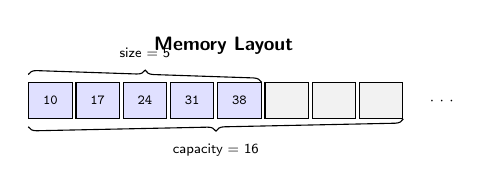
\begin{tikzpicture}[
    cell/.style={draw, minimum width=0.55cm, minimum height=0.45cm,
                 font=\tiny\ttfamily},
    >=Stealth
  ]
  \node[font=\scriptsize\sffamily\bfseries] at (2.2, 1.5)
    {Memory Layout};

  \foreach \i in {0,...,7} {
    \pgfmathsetmacro{\fillcol}{\i < 5 ? "blue!12" : "gray!10"}
    \pgfmathsetmacro{\lbl}{\i < 5 ? int(10+\i*7) : ""}
    \node[cell, fill=\fillcol] (d\i) at (\i*0.6, 0.8) {\lbl};
  }
  \node[font=\tiny\sffamily, right=0.2cm of d7] {$\cdots$};

  \draw[decorate, decoration={brace, amplitude=3pt}]
    (d0.north west) ++(0,0.1) -- (d4.north east) ++(0,0.1)
    node[midway, above=4pt, font=\tiny\sffamily] {size = 5};

  \draw[decorate, decoration={brace, mirror, amplitude=3pt}]
    (d0.south west) ++(0,-0.1) -- (d7.south east) ++(0,-0.1)
    node[midway, below=4pt, font=\tiny\sffamily] {capacity = 16};
\end{tikzpicture}
\end{center}

\vspace{0.3em}
\begin{alertblock}{Static Allocation}
The array is embedded directly in the struct ---
no pointers, no malloc. Capacity is fixed at compile time.
\end{alertblock}
\end{column}
\end{columns}
\end{frame}

% ===========================================================================
\section{API Reference}
% ===========================================================================

\begin{frame}[fragile]{Complete API}
\begin{table}
\centering
\small
\begin{tabular}{@{}lp{8cm}@{}}
\toprule
\textbf{Function} & \textbf{Description} \\
\midrule
\texttt{tiku\_kits\_ds\_sortarray\_init(sa)}
  & Initialize array: set size to 0, capacity to \texttt{MAX\_SIZE} \\
\texttt{tiku\_kits\_ds\_sortarray\_insert(sa, val)}
  & Insert \texttt{val} in sorted position (binary search + memmove right) \\
\texttt{tiku\_kits\_ds\_sortarray\_remove(sa, val)}
  & Remove first occurrence of \texttt{val} (binary search + memmove left) \\
\midrule
\texttt{tiku\_kits\_ds\_sortarray\_find(sa, val)}
  & Return index of \texttt{val} via binary search, or \texttt{ERR\_NOT\_FOUND} \\
\texttt{tiku\_kits\_ds\_sortarray\_contains(sa, val)}
  & Return 1 if \texttt{val} exists, 0 otherwise \\
\texttt{tiku\_kits\_ds\_sortarray\_get(sa, idx, \&out)}
  & Retrieve element at position \texttt{idx} \\
\midrule
\texttt{tiku\_kits\_ds\_sortarray\_min(sa, \&out)}
  & Return minimum (first element, O(1)) \\
\texttt{tiku\_kits\_ds\_sortarray\_max(sa, \&out)}
  & Return maximum (last element, O(1)) \\
\texttt{tiku\_kits\_ds\_sortarray\_clear(sa)}
  & Reset size to 0 \\
\texttt{tiku\_kits\_ds\_sortarray\_size(sa)}
  & Return current number of elements \\
\bottomrule
\end{tabular}
\end{table}

\vspace{0.3em}
\begin{alertblock}{Return Codes}
All mutating functions return \texttt{TIKU\_KITS\_DS\_OK} on success.
Errors: \texttt{ERR\_NULL} (null pointer), \texttt{ERR\_FULL} (capacity reached),
\texttt{ERR\_EMPTY} (array empty), \texttt{ERR\_NOT\_FOUND} (element absent).
\end{alertblock}
\end{frame}

% ===========================================================================
\section{Internal Algorithms}
% ===========================================================================

\begin{frame}[fragile]{Insert Algorithm}
\begin{columns}[T]
\begin{column}{0.52\textwidth}
\begin{lstlisting}[style=cstyle,
  title={Insert: binary search + shift right}]
int tiku_kits_ds_sortarray_insert(
    struct tiku_kits_ds_sortarray *sa,
    tiku_kits_ds_elem_t val)
{
    if (!sa) return TIKU_KITS_DS_ERR_NULL;
    if (sa->size >= sa->capacity)
        return TIKU_KITS_DS_ERR_FULL;

    /* Find insertion position (upper bound) */
    uint8_t lo = 0, hi = sa->size;
    while (lo < hi) {
        uint8_t mid = (lo + hi) / 2;
        if (sa->data[mid] <= val)
            lo = mid + 1;
        else
            hi = mid;
    }

    /* Shift elements right */
    memmove(&sa->data[lo + 1],
            &sa->data[lo],
            (sa->size - lo)
                * sizeof(tiku_kits_ds_elem_t));

    sa->data[lo] = val;
    sa->size++;
    return TIKU_KITS_DS_OK;
}
\end{lstlisting}
\end{column}

\begin{column}{0.44\textwidth}
\begin{center}
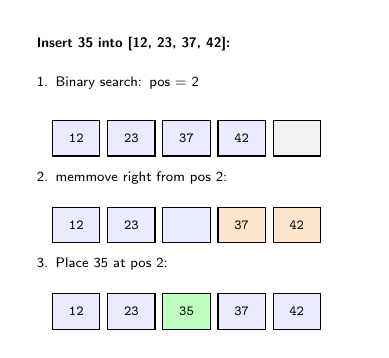
\begin{tikzpicture}[
    cell/.style={draw, minimum width=0.6cm, minimum height=0.45cm,
                 font=\tiny\ttfamily},
    >=Stealth,
    steplbl/.style={font=\tiny\sffamily, text width=4cm}
  ]
  % Step 1: find position
  \node[steplbl, font=\tiny\sffamily\bfseries] at (1.5, 3.2)
    {Insert 35 into [12, 23, 37, 42]:};

  \node[steplbl] at (1.5, 2.7) {1. Binary search: pos = 2};

  % Before shift
  \foreach \v [count=\i from 0] in {12,23,37,42} {
    \node[cell, fill=blue!8] (b\i) at (\i*0.7, 2.0) {\v};
  }
  \node[cell, fill=gray!10] (b4) at (4*0.7, 2.0) {};

  % Arrow showing memmove
  \node[steplbl] at (1.5, 1.5) {2. memmove right from pos 2:};

  \foreach \v [count=\i from 0] in {12,23,,37,42} {
    \pgfmathsetmacro{\fillcol}{\i >= 3 ? "orange!20" : "blue!8"}
    \node[cell, fill=\fillcol] (m\i) at (\i*0.7, 0.9) {\v};
  }

  % Place value
  \node[steplbl] at (1.5, 0.4) {3. Place 35 at pos 2:};

  \foreach \v [count=\i from 0] in {12,23,35,37,42} {
    \pgfmathsetmacro{\fillcol}{\i == 2 ? "green!25" : "blue!8"}
    \node[cell, fill=\fillcol] (a\i) at (\i*0.7, -0.2) {\v};
  }
\end{tikzpicture}
\end{center}

\vspace{0.3em}
\begin{block}{Upper-Bound Search}
Using \texttt{<=} in the binary search ensures duplicates
are inserted \textbf{after} existing equal values, preserving
insertion order among equals.
\end{block}
\end{column}
\end{columns}
\end{frame}

% ---------------------------------------------------------------------------
\begin{frame}[fragile]{Remove Algorithm}
\begin{columns}[T]
\begin{column}{0.52\textwidth}
\begin{lstlisting}[style=cstyle,
  title={Remove: binary search + shift left}]
int tiku_kits_ds_sortarray_remove(
    struct tiku_kits_ds_sortarray *sa,
    tiku_kits_ds_elem_t val)
{
    if (!sa) return TIKU_KITS_DS_ERR_NULL;
    if (sa->size == 0)
        return TIKU_KITS_DS_ERR_EMPTY;

    /* Binary search for the element */
    int idx = tiku_kits_ds_sortarray_find(
        sa, val);
    if (idx < 0)
        return TIKU_KITS_DS_ERR_NOT_FOUND;

    /* Shift elements left */
    memmove(&sa->data[idx],
            &sa->data[idx + 1],
            (sa->size - idx - 1)
                * sizeof(tiku_kits_ds_elem_t));

    sa->size--;
    return TIKU_KITS_DS_OK;
}
\end{lstlisting}
\end{column}

\begin{column}{0.44\textwidth}
\begin{center}
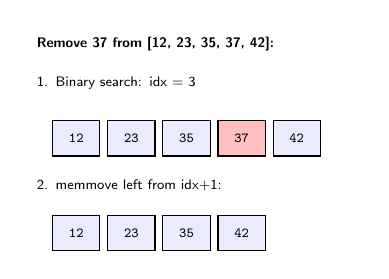
\begin{tikzpicture}[
    cell/.style={draw, minimum width=0.6cm, minimum height=0.45cm,
                 font=\tiny\ttfamily},
    >=Stealth,
    steplbl/.style={font=\tiny\sffamily, text width=4cm}
  ]
  \node[steplbl, font=\tiny\sffamily\bfseries] at (1.5, 2.7)
    {Remove 37 from [12, 23, 35, 37, 42]:};

  \node[steplbl] at (1.5, 2.2) {1. Binary search: idx = 3};

  \foreach \v [count=\i from 0] in {12,23,35,37,42} {
    \pgfmathsetmacro{\fillcol}{\i == 3 ? "red!25" : "blue!8"}
    \node[cell, fill=\fillcol] (b\i) at (\i*0.7, 1.5) {\v};
  }

  \node[steplbl] at (1.5, 0.9) {2. memmove left from idx+1:};

  \foreach \v [count=\i from 0] in {12,23,35,42} {
    \node[cell, fill=blue!8] (a\i) at (\i*0.7, 0.3) {\v};
  }
\end{tikzpicture}
\end{center}

\vspace{0.5em}
\begin{block}{First Occurrence}
\texttt{remove()} deletes the \textbf{first} matching element.
If duplicates exist, subsequent copies remain in the array.
Call \texttt{remove()} repeatedly to remove all occurrences.
\end{block}

\vspace{0.3em}
\begin{alertblock}{memmove Safety}
\texttt{memmove} handles overlapping regions correctly,
unlike \texttt{memcpy}. Essential for in-place shifting.
\end{alertblock}
\end{column}
\end{columns}
\end{frame}

% ===========================================================================
\section{Examples}
% ===========================================================================

\begin{frame}[fragile]{Example 1: Calibration Threshold Lookup}
\begin{lstlisting}[style=cstyle,
  title={examples/example\_ds\_sortarray.c --- ADC threshold lookup}]
struct tiku_kits_ds_sortarray thresholds;
tiku_kits_ds_elem_t val;

tiku_kits_ds_sortarray_init(&thresholds);

/* Load calibration breakpoints (ascending) */
tiku_kits_ds_sortarray_insert(&thresholds, 100);  /* cold */
tiku_kits_ds_sortarray_insert(&thresholds, 200);  /* cool */
tiku_kits_ds_sortarray_insert(&thresholds, 350);  /* warm */
tiku_kits_ds_sortarray_insert(&thresholds, 500);  /* hot  */
tiku_kits_ds_sortarray_insert(&thresholds, 700);  /* critical */

/* Fast lookup: is this reading a known threshold? */
uint16_t adc_reading = read_adc();
if (tiku_kits_ds_sortarray_contains(&thresholds, adc_reading)) {
    trigger_threshold_event(adc_reading);
}

/* Min/max for range checking */
tiku_kits_ds_sortarray_min(&thresholds, &val);  /* val = 100 */
tiku_kits_ds_sortarray_max(&thresholds, &val);  /* val = 700 */

/* Access by index for zone classification */
tiku_kits_ds_sortarray_get(&thresholds, 2, &val);  /* val = 350 */
\end{lstlisting}
\end{frame}

% ---------------------------------------------------------------------------
\begin{frame}[fragile]{Example 2: Alarm Priority Table}
\begin{columns}[T]
\begin{column}{0.52\textwidth}
\begin{lstlisting}[style=cstyle,
  title={Dynamic alarm severity management}]
struct tiku_kits_ds_sortarray alarms;
tiku_kits_ds_elem_t highest;

tiku_kits_ds_sortarray_init(&alarms);

/* Alarms arrive at different times */
tiku_kits_ds_sortarray_insert(&alarms, 3);
tiku_kits_ds_sortarray_insert(&alarms, 7);
tiku_kits_ds_sortarray_insert(&alarms, 1);
tiku_kits_ds_sortarray_insert(&alarms, 5);
/* Array is now: [1, 3, 5, 7] */

/* Highest priority alarm */
tiku_kits_ds_sortarray_max(&alarms, &highest);
/* highest = 7 */

/* Clear resolved alarm */
tiku_kits_ds_sortarray_remove(&alarms, 7);
/* Array is now: [1, 3, 5] */

/* New highest after resolution */
tiku_kits_ds_sortarray_max(&alarms, &highest);
/* highest = 5 */
\end{lstlisting}
\end{column}

\begin{column}{0.44\textwidth}
\begin{center}
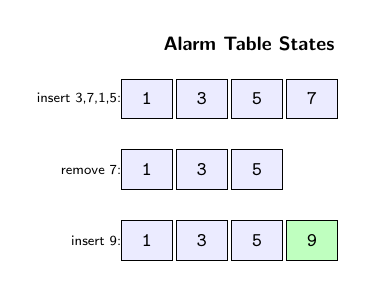
\begin{tikzpicture}[
    cell/.style={draw, minimum width=0.65cm, minimum height=0.5cm,
                 font=\scriptsize\ttfamily},
    lbl/.style={font=\tiny\sffamily},
    >=Stealth
  ]
  \node[font=\scriptsize\sffamily\bfseries] at (1.3, 3.0)
    {Alarm Table States};

  % State 1
  \node[lbl, anchor=east] at (-0.2, 2.3) {insert 3,7,1,5:};
  \foreach \v [count=\i from 0] in {1,3,5,7} {
    \node[cell, fill=blue!8] at (\i*0.7, 2.3) {\v};
  }

  % State 2
  \node[lbl, anchor=east] at (-0.2, 1.4) {remove 7:};
  \foreach \v [count=\i from 0] in {1,3,5} {
    \node[cell, fill=blue!8] at (\i*0.7, 1.4) {\v};
  }

  % State 3
  \node[lbl, anchor=east] at (-0.2, 0.5) {insert 9:};
  \foreach \v [count=\i from 0] in {1,3,5,9} {
    \pgfmathsetmacro{\fillcol}{\i == 3 ? "green!25" : "blue!8"}
    \node[cell, fill=\fillcol] at (\i*0.7, 0.5) {\v};
  }
\end{tikzpicture}
\end{center}

\vspace{0.5em}
\begin{block}{O(1) Min/Max}
Because the array is always sorted, \texttt{min()} returns
\texttt{data[0]} and \texttt{max()} returns
\texttt{data[size-1]} --- both in constant time.
\end{block}
\end{column}
\end{columns}
\end{frame}

% ---------------------------------------------------------------------------
\begin{frame}[fragile]{Example 3: Duplicate Handling}
\begin{columns}[T]
\begin{column}{0.52\textwidth}
\begin{lstlisting}[style=cstyle,
  title={Sorted array with duplicate elements}]
struct tiku_kits_ds_sortarray sa;

tiku_kits_ds_sortarray_init(&sa);

/* Insert duplicates */
tiku_kits_ds_sortarray_insert(&sa, 10);
tiku_kits_ds_sortarray_insert(&sa, 20);
tiku_kits_ds_sortarray_insert(&sa, 20);
tiku_kits_ds_sortarray_insert(&sa, 30);
/* Array: [10, 20, 20, 30] */
/* size = 4 */

/* find() returns first occurrence */
int idx = tiku_kits_ds_sortarray_find(
    &sa, 20);
/* idx = 1 (first 20) */

/* remove() removes first occurrence */
tiku_kits_ds_sortarray_remove(&sa, 20);
/* Array: [10, 20, 30], size = 3 */
\end{lstlisting}
\end{column}

\begin{column}{0.44\textwidth}
\begin{center}
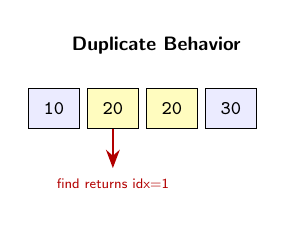
\begin{tikzpicture}[
    cell/.style={draw, minimum width=0.65cm, minimum height=0.5cm,
                 font=\scriptsize\ttfamily},
    >=Stealth
  ]
  \node[font=\scriptsize\sffamily\bfseries] at (1.3, 2.0)
    {Duplicate Behavior};

  \foreach \v [count=\i from 0] in {10,20,20,30} {
    \pgfmathsetmacro{\fillcol}{\i == 1 || \i == 2 ? "yellow!25" : "blue!8"}
    \node[cell, fill=\fillcol] (d\i) at (\i*0.75, 1.2) {\v};
  }

  \draw[->, thick, red!70!black] (d1.south) -- ++(0,-0.5)
    node[below, font=\tiny\sffamily] {find returns idx=1};
\end{tikzpicture}
\end{center}

\vspace{1em}
\begin{block}{Stable Insertion}
New values equal to existing ones are placed \textbf{after}
the last equal element. This makes the insertion stable ---
equal elements maintain their relative insertion order.
\end{block}

\vspace{0.3em}
\begin{alertblock}{Counting Duplicates}
To count occurrences, use \texttt{find()} to locate the first,
then scan forward while values match. Not built-in, but
trivial with \texttt{get()}.
\end{alertblock}
\end{column}
\end{columns}
\end{frame}

% ===========================================================================
\section{Comparison with Other Structures}
% ===========================================================================

\begin{frame}{When to Use Sorted Array vs.\ Others}
\begin{table}
\centering
\small
\begin{tabular}{@{}lccc@{}}
\toprule
\textbf{Property} & \textbf{Sorted Array} & \textbf{Hash Table} & \textbf{B-Tree} \\
\midrule
Lookup           & O($\log n$)    & O(1) avg     & O($\log n$) \\
Insert           & O($n$)         & O(1) avg     & O($\log n$) \\
Remove           & O($n$)         & O(1) avg     & O($\log n$) \\
Min/Max          & O(1)           & O($n$)       & O($\log n$) \\
Ordered iteration & Yes           & No           & Yes \\
Memory overhead  & None           & Load factor  & Node pointers \\
Implementation   & Very simple    & Moderate     & Complex \\
\midrule
\textbf{Best for} & Small, mostly-read & Fast exact lookup & Large, dynamic \\
\bottomrule
\end{tabular}
\end{table}

\vspace{0.5em}
\begin{columns}[T]
\begin{column}{0.48\textwidth}
\begin{block}{Use Sorted Array When\ldots}
\begin{itemize}
  \item Collection is small ($\leq$ 16--32 elements)
  \item Reads far outnumber writes
  \item You need ordered access (min, max, range)
  \item Memory is extremely tight
\end{itemize}
\end{block}
\end{column}

\begin{column}{0.48\textwidth}
\begin{block}{Avoid Sorted Array When\ldots}
\begin{itemize}
  \item Frequent inserts/removes dominate
  \item Collection grows beyond 32 elements
  \item You only need exact-match lookup
  \item Order does not matter
\end{itemize}
\end{block}
\end{column}
\end{columns}
\end{frame}

% ===========================================================================
\section{Test Suite}
% ===========================================================================

\begin{frame}{Test Cases Overview}
\begin{table}
\centering
\small
\begin{tabular}{@{}clp{7cm}@{}}
\toprule
\textbf{\#} & \textbf{Test Function} & \textbf{What It Verifies} \\
\midrule
1 & \texttt{test\_kits\_ds\_sortarray\_init}
  & Proper initialization, size = 0 \\
2 & \texttt{test\_kits\_ds\_sortarray\_insert\_sorted}
  & Elements maintain ascending order after random inserts \\
3 & \texttt{test\_kits\_ds\_sortarray\_insert\_full}
  & Returns \texttt{ERR\_FULL} at capacity \\
4 & \texttt{test\_kits\_ds\_sortarray\_remove}
  & Element removed, remaining elements shifted correctly \\
5 & \texttt{test\_kits\_ds\_sortarray\_find}
  & Binary search returns correct index \\
6 & \texttt{test\_kits\_ds\_sortarray\_contains}
  & Returns 1 for present, 0 for absent \\
7 & \texttt{test\_kits\_ds\_sortarray\_duplicates}
  & Duplicates allowed, find returns first occurrence \\
8 & \texttt{test\_kits\_ds\_sortarray\_min\_max}
  & Min/max correct; \texttt{ERR\_EMPTY} on empty array \\
9 & \texttt{test\_kits\_ds\_sortarray\_clear}
  & Clear resets size to 0 \\
10 & \texttt{test\_kits\_ds\_sortarray\_null\_inputs}
  & All functions reject NULL with \texttt{ERR\_NULL} \\
\bottomrule
\end{tabular}
\end{table}
\end{frame}

% ===========================================================================
\section{Embedded Considerations}
% ===========================================================================

\begin{frame}{Embedded Design Trade-Offs}
\begin{columns}[T]
\begin{column}{0.48\textwidth}
\begin{block}{Advantages}
\begin{itemize}
  \item \textbf{Zero overhead}: no pointers, no metadata per element
  \item \textbf{Cache-friendly}: contiguous memory layout
  \item \textbf{Deterministic}: worst-case is bounded by capacity
  \item \textbf{FRAM-safe}: single contiguous write region
  \item \textbf{Tiny code}: $\sim$200 bytes of flash
\end{itemize}
\end{block}

\begin{block}{FRAM Persistence}
The entire struct can be placed in FRAM with
\texttt{\_\_persistent}. On reboot, the sorted array
is immediately available without re-initialization.
\end{block}
\end{column}

\begin{column}{0.48\textwidth}
\begin{block}{Limitations}
\begin{itemize}
  \item O($n$) insert/remove due to shifting
  \item Fixed capacity at compile time
  \item Not suitable for large collections
  \item No built-in thread safety
\end{itemize}
\end{block}

\begin{block}{Interrupt Safety}
If inserting from an ISR, wrap in a critical section:
\end{block}
\begin{lstlisting}[style=cstyle, basicstyle=\ttfamily\tiny]
/* In ISR context */
__disable_interrupt();
tiku_kits_ds_sortarray_insert(
    &sa, sensor_val);
__enable_interrupt();
\end{lstlisting}
\end{column}
\end{columns}
\end{frame}

% ===========================================================================
\section{Summary}
% ===========================================================================

\begin{frame}{Summary}
\begin{columns}[T]
\begin{column}{0.48\textwidth}
\begin{block}{What We Built}
\begin{itemize}
  \item Statically allocated sorted array
  \item Automatic ascending-order maintenance
  \item O($\log n$) binary search lookup
  \item O(1) min/max access
  \item 66 bytes state (default 16 elements)
  \item Duplicates allowed (stable insertion)
\end{itemize}
\end{block}

\begin{block}{Key Design Choices}
\begin{itemize}
  \item \texttt{memmove} for in-place shifting
  \item Upper-bound search for stable duplicate insertion
  \item No heap, no pointers --- pure array
  \item Configurable capacity via \texttt{MAX\_SIZE}
\end{itemize}
\end{block}
\end{column}

\begin{column}{0.48\textwidth}
\begin{block}{Use Cases}
\begin{itemize}
  \item Calibration threshold lookup
  \item Alarm severity table
  \item Sensor priority ranking
  \item Sorted event scheduling
\end{itemize}
\end{block}

\begin{block}{Files}
\scriptsize
\begin{tabular}{@{}lp{4.5cm}@{}}
Header: & \texttt{ds/sorted/tiku\_kits\_ds\_sortarray.h} \\
Source: & \texttt{ds/sorted/tiku\_kits\_ds\_sortarray.c} \\
Tests: & \texttt{tests/ds/test\_kits\_ds\_sortarray.c} \\
Example: & \texttt{examples/example\_ds\_sortarray.c} \\
\end{tabular}
\end{block}
\end{column}
\end{columns}
\end{frame}

% ---------------------------------------------------------------------------
\begin{frame}{Thank You}
\begin{center}
\Large\textbf{TikuKits DS: Sorted Array}\\[0.5em]
\normalsize Ordered Storage for Resource-Constrained Endpoints\\[1.5em]

\begin{tabular}{rl}
  Repository: & \url{https://github.com/tikuos/tikuOS} \\
  License:    & Apache 2.0 \\
  Common:     & \texttt{tikukits/ds/tiku\_kits\_ds.h} \\
  Header:     & \texttt{tikukits/ds/sorted/tiku\_kits\_ds\_sortarray.h} \\
  Source:     & \texttt{tikukits/ds/sorted/tiku\_kits\_ds\_sortarray.c} \\
  Tests:      & \texttt{tikukits/tests/ds/test\_kits\_ds\_sortarray.c} \\
  Examples:   & \texttt{tikukits/examples/example\_ds\_sortarray.c} \\
\end{tabular}
\end{center}
\end{frame}

\end{document}
